% Figure 3: the plan. The same H-Net reads three kinds of data as bytes.
% The text row is a result; the image and robot rows are hypotheses, drawn dashed.
\documentclass[tikz,border=10pt]{standalone}
\usepackage[T1]{fontenc}
\usepackage[scaled=0.92]{helvet}
\renewcommand{\familydefault}{\sfdefault}
\usetikzlibrary{arrows.meta,calc}

\definecolor{ink}{HTML}{1F1F1E}
\definecolor{quiet}{HTML}{6B6A66}
\definecolor{accent}{HTML}{2A78D6}
\definecolor{accentsoft}{HTML}{E4EEFB}
\definecolor{greysoft}{HTML}{EFEEEA}
\definecolor{greyline}{HTML}{A8A69E}
\definecolor{sky}{HTML}{BFD9F2}
\definecolor{sun}{HTML}{F2C94C}
\definecolor{hill}{HTML}{7FB77E}
\definecolor{hilldark}{HTML}{4F8F5B}
\definecolor{warm}{HTML}{B8742A}

\newcommand{\vsp}{\textcolor{quiet}{\textbullet}}
\newcommand{\cw}{0.30}

% \cells{x left}{y}{labels}: a strip of byte cells with tiny labels
\newcommand{\cells}[3]{%
  \foreach \c [count=\i from 0] in {#3} {%
    \draw[greyline, fill=white, line width=0.45pt]
      ({#1+\i*\cw}, {#2-0.17}) rectangle ({#1+(\i+1)*\cw}, {#2+0.17});
    \node[text=ink, font=\ttfamily\scriptsize, inner sep=0pt] at ({#1+(\i+0.5)*\cw}, {#2}) {\strut\c};
  }%
}

% \chars{x left}{y}{labels}: the same labels without cell borders
\newcommand{\chars}[3]{%
  \foreach \c [count=\i from 0] in {#3} {%
    \node[text=ink, font=\ttfamily\scriptsize, inner sep=0pt] at ({#1+(\i+0.5)*\cw}, {#2}) {\strut\c};
  }%
}

% \cuts{x left}{y}{chunk lengths}{style}: boxes over a strip, one per chunk
\newcommand{\cuts}[4]{%
  \gdef\xoff{0}%
  \foreach \n in {#3} {%
    \draw[rounded corners=2pt, line width=0.7pt, #4]
      ({#1+\xoff*\cw+0.03}, {#2-0.22}) rectangle ({#1+(\xoff+\n)*\cw-0.03}, {#2+0.22});
    \pgfmathtruncatemacro{\next}{\xoff+\n}%
    \xdef\xoff{\next}%
  }%
}

\begin{document}
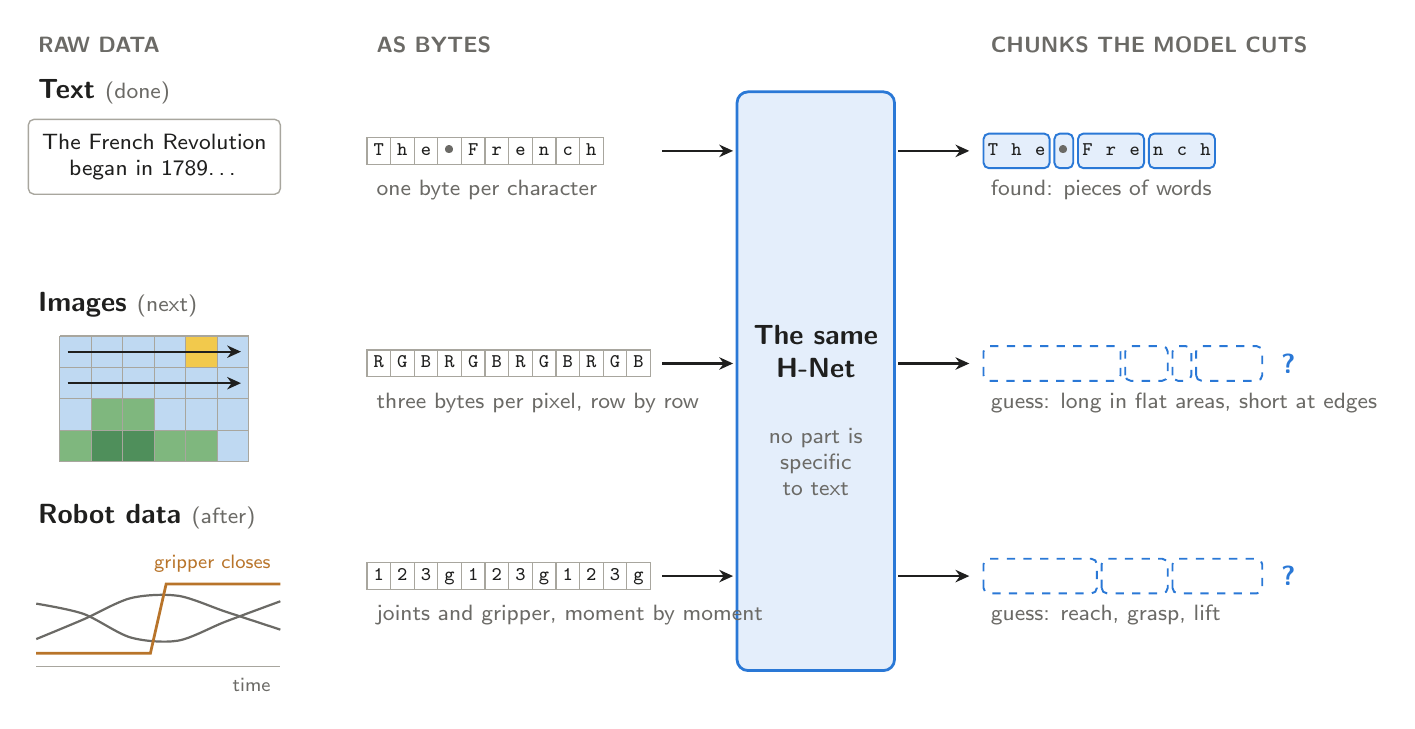
\begin{tikzpicture}[
    >={Stealth[length=5pt,width=4.5pt]},
    flow/.style={->, line width=0.8pt, draw=ink},
    head/.style={anchor=west, font=\bfseries, text=ink},
    small/.style={font=\footnotesize, text=quiet},
    col/.style={font=\footnotesize\bfseries, text=quiet},
  ]
  % x positions: picture 0..3.2, bytes 4.3..7.9, model 9.0..11.0, chunks 12.1..15.7
  % rows at y = 0, -2.7, -5.4

  \node[col, anchor=west] at (0,1.35)    {RAW DATA};
  \node[col, anchor=west] at (4.3,1.35)  {AS BYTES};
  \node[col, anchor=west] at (12.1,1.35) {CHUNKS THE MODEL CUTS};

  % ---------------- the shared model
  \draw[accent, fill=accentsoft, line width=1pt, rounded corners=4pt] (9.0,-6.6) rectangle (11.0,0.75);
  \node[text=ink, font=\bfseries, align=center] at (10.0,-2.55) {The same\\H-Net};
  \node[small, align=center] at (10.0,-3.95) {no part is\\specific\\to text};

  % ---------------- row 1: text (done)
  \node[head] at (0,0.75) {Text {\normalfont\footnotesize\color{quiet}(done)}};
  \draw[greyline, fill=white, line width=0.5pt, rounded corners=2pt] (0,-0.55) rectangle (3.2,0.40);
  \node[text=ink, font=\footnotesize, align=center] at (1.6,-0.075) {The French Revolution\\began in 1789\dots};
  \cells{4.3}{0}{T,h,e,\vsp,F,r,e,n,c,h}
  \node[small, anchor=west] at (4.3,-0.50) {one byte per character};
  \draw[flow] (8.05,0) -- (8.95,0);
  \draw[flow] (11.05,0) -- (11.95,0);
  \cuts{12.1}{0}{3,1,3,3}{draw=accent, fill=accentsoft}
  \chars{12.1}{0}{T,h,e,\vsp,F,r,e,n,c,h}
  \node[small, anchor=west] at (12.1,-0.50) {found: pieces of words};

  % ---------------- row 2: images (next)
  \node[head] at (0,-1.95) {Images {\normalfont\footnotesize\color{quiet}(next)}};
  % a 6 x 4 picture: sky, a sun, a hill
  \foreach \row/\cols in {0/{sky,sky,sky,sky,sun,sky}, 1/{sky,sky,sky,sky,sky,sky},
                          2/{sky,hill,hill,sky,sky,sky}, 3/{hill,hilldark,hilldark,hill,hill,sky}} {
    \foreach \colr [count=\j from 0] in \cols {
      \fill[\colr] ({0.4+\j*0.4}, {-2.35-\row*0.4}) rectangle ++(0.4,-0.4);
    }
  }
  \draw[greyline, line width=0.4pt, step=0.4, shift={(0.4,-2.35)}] (0,0) grid (2.4,-1.6);
  % reading order: row by row
  \draw[->, line width=0.6pt, draw=ink] (0.5,-2.55) -- (2.7,-2.55);
  \draw[->, line width=0.6pt, draw=ink] (0.5,-2.95) -- (2.7,-2.95);
  \cells{4.3}{-2.7}{R,G,B,R,G,B,R,G,B,R,G,B}
  \node[small, anchor=west] at (4.3,-3.20) {three bytes per pixel, row by row};
  \draw[flow] (8.05,-2.7) -- (8.95,-2.7);
  \draw[flow] (11.05,-2.7) -- (11.95,-2.7);
  \cuts{12.1}{-2.7}{6,2,1,3}{draw=accent, dashed}
  \node[text=accent, font=\bfseries] at (16.0,-2.7) {?};
  \node[small, anchor=west] at (12.1,-3.20) {guess: long in flat areas, short at edges};

  % ---------------- row 3: robot data (after)
  \node[head] at (0,-4.65) {Robot data {\normalfont\footnotesize\color{quiet}(after)}};
  % joint values over time, plus the gripper closing
  \draw[greyline, line width=0.5pt] (0.1,-6.55) -- (3.2,-6.55);
  \draw[quiet, line width=0.8pt] plot[smooth] coordinates
    {(0.1,-6.20) (0.7,-5.95) (1.3,-5.68) (1.9,-5.65) (2.5,-5.85) (3.2,-6.08)};
  \draw[quiet, line width=0.8pt] plot[smooth] coordinates
    {(0.1,-5.75) (0.7,-5.88) (1.3,-6.18) (1.9,-6.22) (2.5,-5.98) (3.2,-5.72)};
  \draw[warm, line width=1pt] (0.1,-6.38) -- (1.55,-6.38) -- (1.75,-5.50) -- (3.2,-5.50);
  \node[font=\scriptsize, text=warm, anchor=south east] at (3.2,-5.48) {gripper closes};
  \node[font=\scriptsize, text=quiet, anchor=north east] at (3.2,-6.57) {time};
  \cells{4.3}{-5.4}{1,2,3,g,1,2,3,g,1,2,3,g}
  \node[small, anchor=west] at (4.3,-5.90) {joints and gripper, moment by moment};
  \draw[flow] (8.05,-5.4) -- (8.95,-5.4);
  \draw[flow] (11.05,-5.4) -- (11.95,-5.4);
  \cuts{12.1}{-5.4}{5,3,4}{draw=accent, dashed}
  \node[text=accent, font=\bfseries] at (16.0,-5.4) {?};
  \node[small, anchor=west] at (12.1,-5.90) {guess: reach, grasp, lift};
\end{tikzpicture}
\end{document}
